\documentclass[solutionorbox, answers]{exam}

%%%%%%%%%%%%%%%%%%%%%%%%%%%%%%%%%%%%%%%%%%%%%%%%%%%%%%%%%%%%%%%
% Update to change header
\newcommand{\courseName}{CS 577}
\newcommand{\assignmentName}{Assignment 6 -- Divide and Conquer 2}
\newcommand{\semester}{Spring 2023}
%%%%%%%%%%%%%%%%%%%%%%%%%%%%%%%%%%%%%%%%%%%%%%%%%%%%%%%%%%%%%%%

\usepackage[utf8]{inputenc}
\usepackage[T1]{fontenc}

\usepackage{amsmath}
\usepackage{amsfonts}
\usepackage{amsthm}
\usepackage{booktabs}
\usepackage{tkz-graph}
\usepackage[ruled]{algorithm2e}
\usepackage{graphicx}
\usepackage{enumitem}
\usepackage{paracol}

%\usepackage{wrapfig}

\usepackage{hyperref}

\pagestyle{headandfoot}
\runningheadrule
\firstpageheader{\courseName}{\huge \assignmentName}{\semester}
\runningheader{\courseName}
{\assignmentName}
{\semester}
\firstpagefooter{}{}{}
\runningfooter{}{Page \thepage\ of \numpages}{}

\begin{document}

\begin{center}
\fbox{\parbox{5.5in}{\centering
Answer the questions in the boxes provided on the
question sheets. If you run out of room for an answer,
add a page to the end of the document. \\
\vspace{0.1in}
}}
\end{center}
\vspace{0.1in}
\makebox[0.48\textwidth]{Name:\enspace\hrulefill} \qquad
\makebox[0.48\textwidth]{Wisc id:\enspace\hrulefill}

\begin{questions}

\section*{Divide and Conquer}

\question
\emph{Kleinberg, Jon. Algorithm Design (p. 248, q. 5)} Hidden surface removal is a problem in computer graphics where you identify objects that are completely hidden behind other objects, so that your renderer can skip over them. This is a common graphical optimization.

In a clean geometric version of the problem, you are given $n$ non-vertical, infinitely long lines in a plane labeled $L_1\ldots L_n$. You may assume that no three lines ever meet at the same point. (See the figure for an example.) We call $L_i$ ``uppermost'' at a given $x$ coordinate $x_0$ if its $y$ coordinate at $x_0$ is greater than that of all other lines. We call $L_i$ ``visible'' if it is uppermost for at least one $x$ coordinate.

\vspace*{-2ex}
\begin{center}
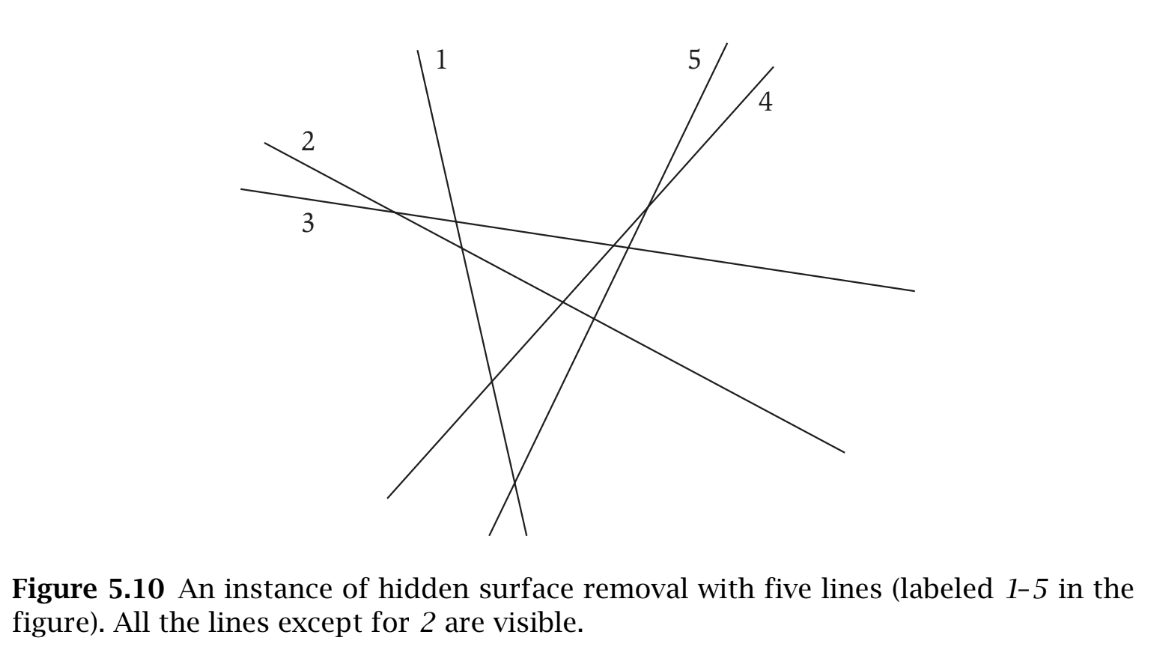
\includegraphics[width=0.7\textwidth]{LineRemoval.png}
\end{center}

\vspace*{-20ex}
\hspace*{20ex}
\begin{tikzpicture}[->]
    \draw (0,0) -- (xyz cs:x=1) node[anchor=north west] {$x$};
    \draw (0,0) -- (xyz cs:y=1) node[anchor=south east] {$y$};
\end{tikzpicture}
\vspace*{5ex}

\begin{parts}
\part Give an algorithm that takes $n$ lines as input and in $O(n\log n)$ time returns all the ones that are visible. 
\begin{solutionbox}{\stretch{1}}

\end{solutionbox}

\newpage
\part Write the recurrence relation for your algorithm.
\begin{solutionbox}{\stretch{1}}

\end{solutionbox}

\part Prove the correctness of your algorithm.
\begin{solutionbox}{\stretch{1}}

\end{solutionbox}

\end{parts}


\newpage
\question In class, we considered a divide and conquer algorithm for finding the closest pair of points in a plane. Recall that this algorithm runs in $O(n\log n)$ time. Let's consider two variations on this problem:

\begin{parts}
\part First consider the problem of searching for the closest pair of points in 3-dimensional space. Show how you could extend the single plane closest pairs algorithm to find closest pairs in 3D space. Your solution should still achieve $O(n\log n)$ run time.
\begin{solutionbox}{2in}

\end{solutionbox}

\part Now consider the problem of searching for the closest pair of points on the surface of a sphere (distances measured by the shortest path across the surface). Explain how your algorithm from part a can be used to find the closest pair of points on the sphere as well.
\begin{solutionbox}{\stretch{1}} 


\end{solutionbox}

\part Finally, consider the problem of searching for the closest pair of points on the surface of a torus (the shape of a donut). A torus can be thought of taking a plane and ``wrap'' at the edges, so a point with $y$ coordinate MAX is the same as the point with the same $x$ coordinate and $y$ coordinate MIN. Similarly, the left and right edges of the plane wrap around. Show how you could extend the single plane closest pairs algorithm to find closest pairs in this space.

\begin{solutionbox}{\stretch{1}} 

\end{solutionbox}

\end{parts}
\newpage
\question \emph{Erickson, Jeff. Algorithms (p. 58, q. 25 d and e)} Prove that the following algorithm computes gcd($x,y$) the greatest common divisor of $x$ and $y$, and show its worst-case running time.
\begin{verbatim}
BINARYGCD(x,y):
if x = y:
    return x
else if x and y are both even:
    return 2*BINARYGCD(x/2,y/2)
else if x is even:
    return BINARYGCD(x/2,y)
else if y is even:
    return BINARYGCD(x,y/2)
else if x > y:
    return BINARYGCD( (x-y)/2,y )
else
    return BINARYGCD( x, (y-x)/2 )
\end{verbatim}

\begin{solutionbox}{2in}


\end{solutionbox}
\question Here we explore the structure of some different recursion trees than the previous homework.
\begin{parts}
% part a
\part Asymptotically solve the following recurrence for $A(n)$ for $n\geq 1$.
\[
    A(n) = A(n/6) + 1
    \qquad \text{with base case} \qquad
    A(1) = 1
\]
\begin{solutionbox}{2in}


\end{solutionbox}

\newpage
% part b
\part Asymptotically solve the following recurrence for $B(n)$ for $n\geq 1$.
\[
    B(n) = B(n/6) + n
    \qquad \text{with base case} \qquad
    B(1) = 1
\]
\begin{solutionbox}{\stretch{1}}


\end{solutionbox}
% part c
\part Asymptotically solve the following recurrence for $C(n)$ for $n\geq 0$.
\[
    C(n) = C(n/6) + C(3n/5) + n
    \qquad \text{with base case} \qquad
    C(0) = 0
\]
\begin{solutionbox}{\stretch{1}}


\end{solutionbox}
% part d
\part Let $d>3$ be some arbitrary constant.  Then solve the following recurrence for $D(x)$ where $x\geq 0$.
\[
    D(x) = D\left(\tfrac{x}{d}\right)
    +
    D\left(\tfrac{(d-2)x}{d}\right)
    +
    x
    \qquad \text{with base case} \qquad
    D(0) = 0
\]
\begin{solutionbox}{\stretch1}


\end{solutionbox}
\end{parts}

\newpage
\question Implement a solution in either C, C++, C\#, Java, Python, or Rust to the following problem.

Suppose you are given two sets of $n$ points, one set $\{p_1, p_2, \ldots, p_n\}$ on the line $y=0$ and the other set $\{q_1, q_2, \ldots, q_n\}$ on the line $y=1$. Create a set of $n$ line segments by connecting each point $p_i$ to the corresponding point $q_i$. Your goal is to develop an algorithm to determine how many pairs of these line segments intersect. Your algorithm should take the $2n$ points as input, and return the number of intersections. Using divide-and-conquer, you should be able to develop an algorithm that runs in $O(n \log{n})$ time.  \\ \textit{Hint:} What does this problem have in common with the problem of counting inversions in a list?

Input should be read in from stdin. The first line will be the number of instances. For each instance, the first line will contain the number of pairs of points ($n$). The next $n$ lines each contain the location $x$ of a point $q_i$ on the top line. Followed by the final $n$ lines of the instance each containing the location $x$ of the corresponding point $p_i$ on the bottom line. For the example shown in Fig~\ref{fig:input}, the input is properly formatted in the first test case below.

\begin{figure}[h]
\begin{center}
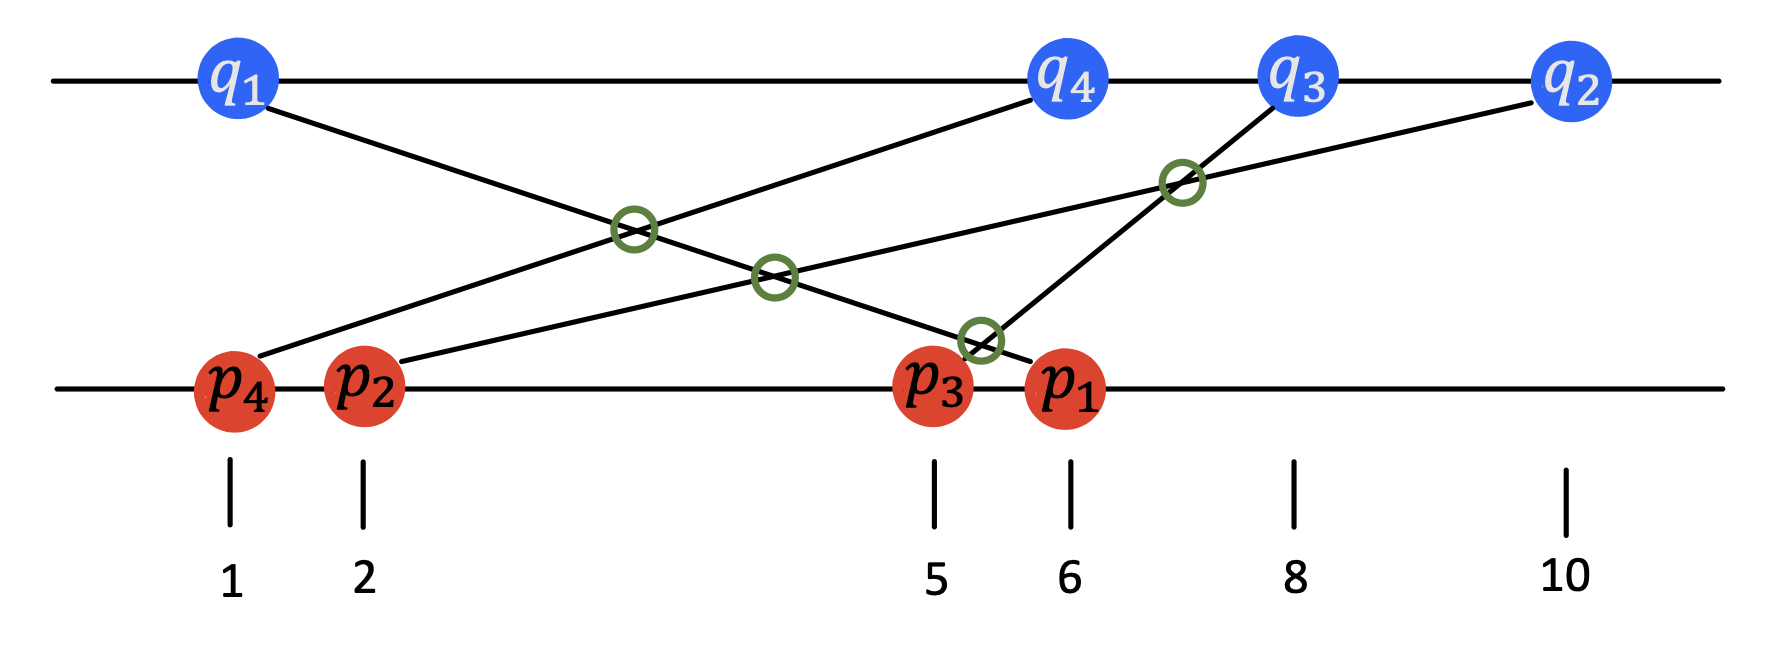
\includegraphics[width=10cm]{input.png}
\caption{An example for the line intersection problem where the answer is 4}
\label{fig:input}
\end{center}
\end{figure}

\medskip
\noindent\textbf{Constraints:}
\begin{itemize}[noitemsep,topsep=0pt]
    \item $1 \leq n \leq 10^6$
    \item For each point, its location $x$ is a positive integer such that $1 \leq x \leq 10^6$
    \item No two points are placed at the same location on the top line, and no two points are placed at the same location on the bottom line.
    \item Note that in C\textbackslash C++, the results of some of the test cases may not fit in a 32-bit integer. If you are using C\textbackslash C++, make sure you use a `long long' to store your final answer.
\end{itemize}


\newpage
\noindent\textbf{Sample Test Cases:} \\

\noindent input:
\\2 \\ 4 \\ 1 \\ 10 \\ 8 \\ 6 \\ 6 \\ 2 \\ 5 \\ 1 \\ 5 \\ 9 \\ 21 \\ 1 \\ 5 \\ 18 \\ 2 \\ 4 \\ 6 \\ 10 \\ 1 \\

\noindent expected output: \\ 4 \\ 7

\end{questions}

\end{document}